%File: formatting-instruction.tex
\documentclass[letterpaper]{article}
% AAAI format packages
\usepackage{aaai}
\usepackage{times}
\usepackage{helvet}
\usepackage{courier}
% Additional packages
\usepackage{amsmath}
\usepackage{amssymb}
\usepackage{amsthm}
\usepackage{algorithm}
\usepackage{algorithmic}
\usepackage{graphicx}
\newtheorem{thm}{Theorem}
\newtheorem{defn}{Definition}
% END Additional packages
\frenchspacing
\setlength{\pdfpagewidth}{8.5in}
\setlength{\pdfpageheight}{11in}
\pdfinfo{
/Title (Experience-Biased Symbolic Planning)
/Author (Aram Ebtekar, Mike Phillips, Maxim Likhachev, Sven Koenig)
/Keywords (symbolic planning, E-graph, experience-biasedh, A* search, STRIPS, HSP)
}
\setcounter{secnumdepth}{0}  
 \begin{document}
% The file aaai.sty is the style file for AAAI Press 
% proceedings, working notes, and technical reports.
%
\title{Experience-Biased Symbolic Planning}
\author{Aram Ebtekar \and Mike Phillips \and Maxim Likhachev\\
Carnegie Mellon University\\
5000 Forbes Ave,\\
Pittsburgh, PA 15213\\
\And Sven Koenig\\
University of Southern California\\
Los Angeles, CA 90089
}
\maketitle
\begin{abstract}
\begin{quote}
Weighted A* search is the foundation for state-of-the-art domain-independent symbolic planners.
An important open challenge for these planners is to utilize experience with similar planning problems to speed up subsequent planning episodes.
Experience graphs have recently shown promise as a technique for plan reuse in the context of weighted A* searches in robotics, by biasing them towards a subgraph of the search space, typically chosen to consist of the edges used in previous plans.
In this paper, we demonstrate how to augment symbolic planners with
experience graphs, using the HSP STRIPS planner as a representative
example.
The resulting planners are able to trade off seamlessly
between plan quality and runtime and thus have advantages over past
plan-reuse techniques, such as planning by analogy.
We demonstrate
experimentally that our planner speeds up HSP by a factor of 2 or more on
many domains while achieving about the same plan quality.
\end{quote}
\end{abstract}

\section{Introduction}
Planning entails finding action sequences that achieve a goal state.
In order to apply the language of graph theory, states are often thought of as nodes connected by action transitions.
A \textbf{plan} is a path from the start state to one of many goal states.
Despite the existence of classic polynomial-time search techniques, such as Dijkstra's algorithm, planning remains the crux of many difficult problems in AI.

The reason usually is that the graphs involved are very large; indeed, too large for explicit storage.
In motion planning, the state space may be a continuous geometric set whose desired discretization is very fine.
In symbolic planning, a planning language such as STRIPS, SAS+, ADL or PDDL [CITE] is chosen to give a compressed symbolic representation.

The graph is exponentially larger than its encoding so, in both cases, states are generated only as needed.
The compressed representation sometimes encodes exploitable structure.
In order to create a domain-independent solver for a language such as STRIPS, we need to automatically extract and interpret structural information about the problem. 

We may view planning as a process that generates distance-to-goal labels for each node of a graph.
Given these distance labels, it's a simple matter to generate a plan by tracing steps from the start, successively taking the optimal successor.
Since there is no worst-case polynomial-time algorithm that can solve the shortest-paths problem in STRIPS (recall the graph is exponential-sized), we may try to roughly approximate the distance labels.

The approximate labels we call \textbf{heuristics}, and we use them in hopes of finding plans more efficiently.
If the heuristic precisely reflects the true distances, we can immediately retrieve a path.
Algorithms such as A* are designed to find solutions quickly whenever the heuristic is of reasonable quality.
If we hope to take subexponential time, we can only afford to examine a vanishing fraction of the states, and it is only for these that we compute the heuristic.
If the heuristic is good, we hope not to have to look at (i.e. generate) too many states.
Hence, there is a tradeoff between spending more time to compute a more accurage heuristic, vs evaluating a weaker heuristic quickly but at many more states.

In practice, even using state-of-the-art methods to generate heuristics on isolated planning instances, STRIPS problems can be very difficult to solve without domain knowledge.
Even humans have difficulty when faced with an unfamiliar kind of puzzle, though we get better with experience.
Thus, one might hope that a planning agent would similarly learn to generalize solutions from past planning experiences to related new instances.
A recent approach builds \textbf{Experience graphs} to estimate the high-level connectivity of the free space in motion planning tasks \cite{phillips2012graphs}.
The intuition is to remember previously generated paths so that, when a new start and goal is queried, a new path can be quickly generated by reusing subpaths from the E-graph.
However, E-graphs have never before been applied to high-level representations such as STRIPS. This is our present contribution.

In section [???], we present the HSP heuristic for STRIPS.
Then, we discuss E-graphs in more technical detail.
This paper's novel contributions follow thereafter, where we extend E-graphs to STRIPS planning by using it to augment the HSP heuristic. 
The resulting A* search is complete with a configurable suboptimality guarantee.
Finally, we present experiment results in which this use of E-graphs is demonstrated to achieve considerable speedups over experience-free HSP in several planning domains.

\section{Related Work}

\section{STRIPS Language}

A STRIPS problem is a tuple $P = \langle A,O,I,G\rangle$ consisting of an atom set $A$, operator set $O$, initial state $I \subseteq A$ and goal condition $G \subseteq A$.
Each operator $op\in O$ is defined by its cost, preconditions, add effects and delete effects: $Cost(op) \in \mathbb{R}^+$ and $Prec(op),Add(op),Del(op) \subseteq A$.

The problem $P$ defines a directed state graph $(V,c)$ where $V$ is the power set of $A$ (i.e. states $S\in V$ correspond to collections of atoms), and the edge costs are
\begin{eqnarray*} c(S,S') = \min\{Cost(op) \mid S\subseteq Prec(op)\text{ and}
\\S' = \left(S \setminus Del(op)\right) \cup Add(op)\} \end{eqnarray*}
%consists of states transitions $(u,v)$ for which there exists an operator $op\in O$ with $u\in Prec(op)$ and $v = u - Del(op) \cup Add(op)$; the weight of this edge is the minimum cost of such an $op$.
By default, $c(S,S') = \infty$ when there is no operator directly transitioning from $S$ to $S'$.
Given a STRIPS problem $P$, we seek a low-cost path from the initial state $I\in V$ to any of the goal states $S\in V$ such that $S \supset G$.

\section{HSP Heuristic}

Many of today's state-of-the-art domain-independent STRIPS planners are based on the HSP planner \cite{bonet2001planning}, which we now describe.
It's common to compute heuristics by solving an easier, relaxed version of the original problem. In STRIPS, one might ignore the delete lists of operations.
Since having more atoms makes preconditions and the goal condition more likely to hold, this can only make the problem easier, so the resulting heuristic never overestimates the true cost.

However, even the relaxed STRIPS planning problem includes set-cover as a special case, making it NP-hard.
Intuitively, we see that the relaxed search space remains exponential.
To reduce it, HSP decouples the atoms, instead estimating the cost of achieving each individual atom.

Let's say we want a heuristic estimate of the distance from $S$ to a goal that contains $G$. HSP estimates the cost to achieve an atom $a\in A$ from $S$ by $g_S(a) = $
\[\begin{cases} 0  &\mbox{if } a \in S
\\ \min_{op\mid a\in Add(op)} \left(g_S(Prec(op)) + Cost(op)\right)  &\mbox{if } a \notin S \end{cases}\]

The HSP heuristic is then defined by
\[h^{HSP}(S) = g_S(G),\]
the estimated cost of achieving all atoms in $G$. Note that $g_S(\cdot)$ is evaluated on certain atom sets, namely $Prec(op)$ and $G$.
To keep the computations feasible, define $g_S(P) = \max_{p\in P} g_S(p)$ for atom sets $P$.
The resulting HSP-max heuristic is an underestimate; indeed, it satisfies a stronger property called \textbf{consistency}.

\begin{defn} For $\epsilon\ge 1$, a heuristic $h$ is called \textbf{$\epsilon$-consistent} if $h(S) = 0$ when $S$ is a goal and $h(S) \le \epsilon c(S,S') + h(S')$ for all $S,S'\in V$. $h$ is \textbf{consistent} if it is $1$-consistent. \end{defn}
\begin{thm} Given an $\epsilon$-consistent heuristic and expanding no node more than once, A* is guaranteed to find a path costing no more than $\epsilon$ times the optimal path cost.  \end{thm}

If the atoms were truly independent, a more accurate estimate would be $g_S(P) = \sum_{p\in P} g_S(p)$.
Despite its inconsistency in general, the latter HSP-plus heuristic is often useful in practice, as it uses more information and biases more greedily toward the goal.

From a computational perspective, the HSP heuristic must compute $g_S(a)$ for all $a\in A$ whenever a new state $S$ is generated.
This can be done by dynamic programming, iterating the recursive formula to a fixpoint in Bellman-Ford-like fashion.
In a sense, it seems we are wasting a lot of work by estimating the cost to reach every atom when we only require $g_S(G)$.
Later, we'll see how to make better use of this computation.

\section{Experience Graphs}

E-graphs can improve total search time over a series of related queries on the same graph.
Formally, an E-graph is a subgraph of the state space.
We update it between queries, typically by adding the solution path from the previous search query.

Suppose we have a consistent heuristic $h(S,S')$ for the distance between arbitrary pairs of states.
That is, $h$ obeys the triangle inequality with respect to edge costs, and $h(S,S) = 0$ for all $S\in V$.
The E-graph heuristic $h^E$ biases the search to follow E-Graph edges instead of $h$ by penalizing the latter by an inflation factor $\epsilon^E > 1$.
To be precise, define

\[h^E(S_0) = \min_{N,S_N,\pi} \sum_{i=1}^N \min \{\epsilon^E h(S_{i-1},S_i),c^E(S_{i-1},S_i)\}\]
over all goal states $S_N$ and paths $\pi = \langle S_0,S_1,...,S_N \rangle$.

$c^E$ are E-graph edge costs, or $\infty$ if the E-graph edge does not exist.

In the limit as $\epsilon^E \rightarrow 1$, following E-graph edges offers no advantage as $h$ is already an underestimate. Hence, using the triangle inequality to coalesce the sum,
\[h^E(S_0) = \min_{N,S_N,\pi} \sum_{i=1}^N h(S_{i-1},S_i) = \min_{S_N} h(S_0,S_N)\]

Conversely as $\epsilon^E \rightarrow\infty$, the cost remains bounded iff $S_0$ is in an E-graph component which also contains a goal state, and the minimizing path becomes the one which uses the fewest edges outside the E-graph.

We cannot afford to compute $h^E$ according to its literal definition, as there are far too many paths to consider. Fortunately, there exists a practical means of computing it. By the triangle inequality, any consecutive pair of $h(S_{i-1},S_i)$ terms can be merged into one. Thus we lose no generality in restricting $S_i$ to lie on the E-graph for $0 < i < N$.

Let $V^E$ be the union of the goal states and the E-graph's vertices.
In addition to following E-graph edges, we imagine it's possible to ``jump" from $S$ to $S'$ with cost $\epsilon^E h(S,S')$. That is, let $c'(S,S') = \min\left(c(S,S'),~\epsilon^E g_S(S')\right)$


In a preprocessing stage before the main search, we apply Dijkstra's algorithm once in reverse with the costs $c'$ to compute the estimated distance-to-goal $h^E(S)$ from every $S\in V^E$. If the blackbox heuristic $h$ is cheap to compute, this preprocessing takes $O(|V^E|^2)$ time, which is negligible for small E-graphs.

Later, when generating $S \notin V^E$, we see that we have already precomputed costs of paths consisting of all but the first edge of $\pi$ according to the definition of $h^E(S)$. Thus, we derive the mathematically equivalent but much cheaper computation
\[h^E(S) = \min_{S'\in V^E} \left(\epsilon^E h(S,S') + h^E(S')\right)\]

\begin{thm}$h^E$ is $\epsilon^E$-consistent. \cite{phillips2012graphs}\end{thm}

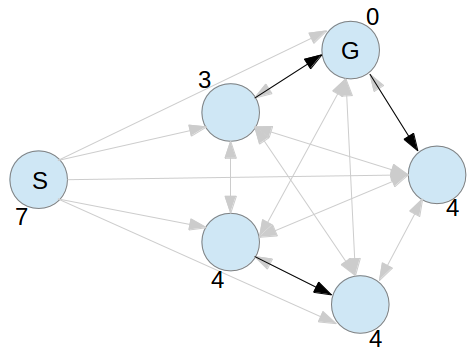
\includegraphics[scale=0.4]{Pentagon.png}

The above figure illustrates the idea. Suppose the dark edges have cost 3 and make up the E-graph. Non-E-graph edges are not shown; instead, light edges represent the jump estimates $h(S_i,S_j) = 2$ (with one exception: $h(S,G) = 5$), which we inflate by a factor $\epsilon^E=2$ to make 4 (or 10, respectively). Dijkstra's algorithm follows the edges backward to compute the $h^E$ values shown alongside each node.

$G$ is on the E-graph, though this need not be the case in general. $V^E$ is the pentagon on the right, and its $h^E$ values are precomputed before the search. $h^E(S)$ is computed only when A* generates $S\notin V^E$.

\section{Experience-Biased HSP}

Now we combine the ideas from HSP and E-graphs to construct a domain-independent STRIPS planner which learns from experience. In STRIPS, a consistent heuristic $h(S,S')$ is given by the HSP-max estimate $h^{HSP}_S(S')$. We can compute $h^{HSP}_S(S')$ for all $S,S'\in V^E$ in precisely $|V^E|$ runs of the dynamic programming we saw before: each run gives us $|V^E|$ of these results, yielding $(|V^E|)^2$ values in total.

Thus, our preprocessing work is roughly equivalent to that of generating $|V^E|$ states, which will be small. As before, Dijkstra's algorithm combines an inflation of these estimates with the E-graph edges to derive $h^E(S)$ for all $S\in V^E$. Note that in STRIPS, $V^E$ need not include every goal state: the minimal goal $G$ suffices as it's always the easiest to reach in the heuristic relaxation.

Upon encountering a new state $S\notin V^E$, we run dynamic programming procedure again to compute $g_S(a)$ for all atoms $a\in A$. Then it's a simple matter to compute the E-graph heuristic by

\[h^E(S) = \min_{S'\in V^E} \left( \epsilon^E g_S(S') + h^E(S') \right)\]

We remark that, when E-graphs are involved, the values $g_S(S')$ on the right-hand side range over a variety of different states $S'$. Compare this to the formula for $h^{HSP}$, which uses only $g_S(G)$. HSP would still compute all the $g_S$-values despite using them only once, so here we get to consult the E-graph essentially for free. The only additional work is the minimization over $S'\in V^E$, which is negligible for small E-graphs. A pseudocode implementation is listed in Algorithms \ref{alg:ComputeG} and \ref{alg:Search}. The parameter $\epsilon^E$ controls bias toward the E-graph, while $\epsilon$ provides an additional goal-directed bias.

\begin{algorithm}
\caption{ComputeG(S)}
\label{alg:ComputeG}
\begin{algorithmic}
\FORALL{$a \in A$}
\IF{$a \in S$}
\STATE $g_S(a) \leftarrow 0$
\ELSE
\STATE $g_S(a) \leftarrow \infty$
\ENDIF
\ENDFOR
\REPEAT
\FORALL{$op \in O$}
\STATE $pCost \leftarrow g_S(Prec(op))$
\FORALL{$a \in Add(op)$}
\STATE $g_S(a) \leftarrow \min \left(g_S(a),~pCost + Cost(op)\right)$
\ENDFOR
\ENDFOR
\UNTIL{no further change in $g$-values}
\end{algorithmic}
\end{algorithm}

\begin{algorithm}
\caption{Search()}
\label{alg:Search}
\begin{algorithmic}
\STATE Let $c(S,S')$ for $S,S'\in V^E$ represent E-graph edge costs.
\FORALL{$S \in V^E$}
\STATE ComputeG(S)
\FORALL{$S' \in V^E$}
\STATE $c'(S,S') \leftarrow \min\left(c(S,S'),~\epsilon^E g_S(S')\right)$
\ENDFOR
\ENDFOR
\STATE Compute $h^E$ on $V^E$ by reverse Dijkstra from $G$ with $c'$.
\STATE Run A* on the full graph from $I$ with heuristic $\epsilon h^E$:
\FOR{$S \notin V^E$ when generated by A*}
\STATE ComputeG(S)
\STATE $h^E(S) \leftarrow \min_{S'\in V^E} \left( \epsilon^E g_S(S') + h^E(S') \right)$
\ENDFOR
\IF{A* successfully found a path to some goal state $S \supseteq G$}
\STATE Add all edges of the solution path to the E-graph.
\RETURN solution path
\ELSE
\RETURN failure
\ENDIF
\end{algorithmic}
\end{algorithm}

ComputeG implements the dynamic programming computation of $g$-values.
Each iteration of the outermost loop permanently fixes at least one $g_S(a)$ value, so it does at most $|A|+1$ iterations.
Multiplying everything together and ignoring cardinality signs for brevity, the runtime bound is $O(\mathbf{A^2O})$.
Thus, each state generated costs $O(\mathbf{A^2O + V^E})$ time.
The preprocessing cost is $O(\mathbf{A^2OV^E + (V^E)^2})$, asymptotically equivalent to preemptively generating every state in $V^E$.
For comparison, standard HSP without E-graphs takes $O(\mathbf{A^2O})$ time (with essentially the same constant factors) to generate a state, and does not incur the cost of generating a state unless the A* encounters it.

\begin{thm}
Provided there exists a path from initial state $I$ to a goal state $S\supseteq G$, the experience-biased HSP algorithm finds a path which is at most $\epsilon\epsilon^E$-suboptimal.
\end{thm}

This follows directly from Theorems 1 and 2, since the weighted heuristic $\epsilon h^E$ is $\epsilon \epsilon^E$-consistent.
However, E-graphs make no guarantee of improving the search time. Indeed, biasing toward bad regions could trap the planner inside large local optima.
Potential gains depend entirely on choosing a good small set of edges to form our E-graph.
In our experiments, we simply keep the previous solution path; different choices remain a topic for future investigations.

\section{Experimental Setup}

We augmented the HSP planner code \cite{bonet2001planning} which won [AI COMPETITION IN 2000] with E-graphs. Our aim is to observe the effect of E-graphs on planning time given that we've already solved a closely related problem. To measure this, we run three searches for each problem instance. First, we run the original problem using standard HSP. Then, we generate a modified problem by moving the start and goal nodes randomly for X steps each. The second search solves the modified problem in the standard way. Finally, the third search solves the modified problem using as E-graph a random Y\% of the path obtained from the first search. The reason for saving only a portion of the previous experience is to simulate the effects of disconnected E-graphs, as might arise after multiple searches. Our main comparisons will be between the number of nodes generated in the second and third searches. In practice, the times followed similar ratios to the number of nodes generated; as one would expect from the analyis in [PREVIOUS SECTION] since the E-graph resulting from Y\% of a single path is very small.

\section{Experimental Results}

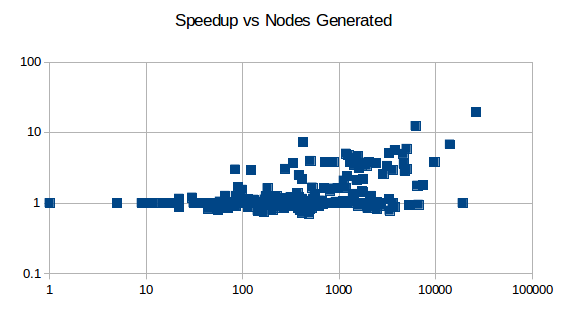
\includegraphics[scale=0.4]{AIPlot.png}

The plot shows speedup (i.e. ratio of nodes generated in the second and third searches) against a measure of problem size (i.e. nodes generated in the second search). Planning times followed similar trends as node generation counts, as one would expect from the analyis since the E-graph resulting from a half-path is very small. We see considerable speedups in many domains, while the plan costs stayed roughly the same (in fact, they became slightly shorter on average). Many domains saw no discernable effect, but none were significantly hurt by E-graphs.

\begin{center}
    \begin{tabular}{| l | l | l | l |}
    \hline
    Domain & 0 steps & 10 steps & 20 steps
    \\ \hline
    BlocksWord & 0 & 0 & 0
    \\ \hline
    Grid & 0 & 0 & 0
    \\ \hline
    Satellite & 0 & 0 & 0
    \\ \hline
    \end{tabular}
\end{center}

\section{Conclusions and Extensions}

We saw that by reusing pieces from past plans, planning time can often be reduced. Many interesting directions remain for future investigation. The E-graph cannot be allowed to grow without bound over countless planning episodes, so a better scheme is needed for expansion and pruning as the agent learns.

Distinct states in STRIPS can actually be very similar, differing only by a few irrelevant atoms; hence, experiences should be transferable to inexact matches.

What if graph changes? Anytime incremental...

\bibliographystyle{aaai}
\bibliography{paper.bib}

\end{document}
